\documentclass[problem]{mcs}

\begin{pcomments}
  \pcomment{PS_tetris_recurrence_well_order}
  \pcomment{F03.rec2 using induction}
  \pcomment{ARM revised for WOP 2/3/17}
\end{pcomments}

\pkeywords{
  recurrence
  tetris
  tiling
}

%%%%%%%%%%%%%%%%%%%%%%%%%%%%%%%%%%%%%%%%%%%%%%%%%%%%%%%%%%%%%%%%%%%%%
% Problem starts here
%%%%%%%%%%%%%%%%%%%%%%%%%%%%%%%%%%%%%%%%%%%%%%%%%%%%%%%%%%%%%%%%%%%%%

\begin{problem}
A {\em winning configuration} in the game of Mini-Tetris is a complete
tiling of a $2 \times n$ board using only the three shapes shown
below:

\bigskip
\centerline{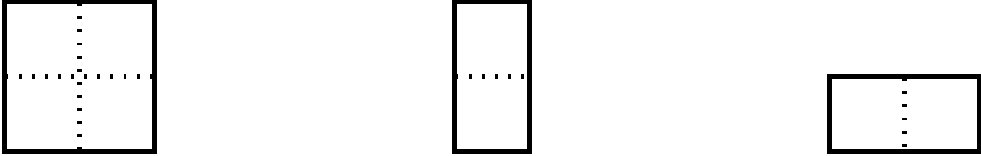
\includegraphics[height=0.5in]{rec2-tetrispieces}}
\bigskip

For example, here are several possible winning configurations on a $2
\times 5$ board:

\bigskip
\centerline{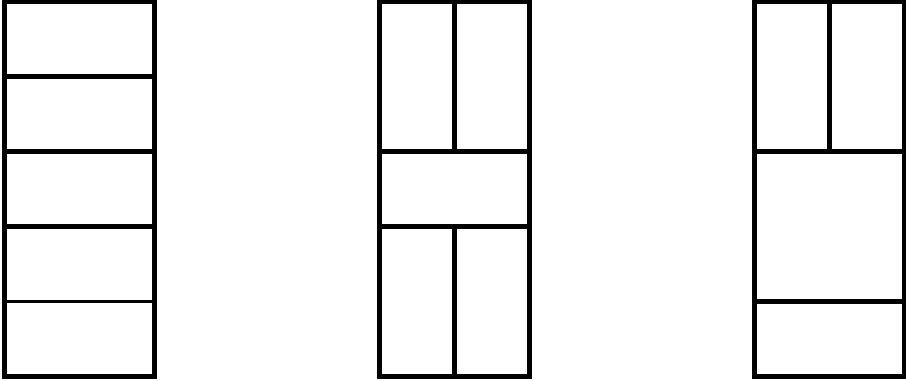
\includegraphics[height=1.25in]{rec2-2x5wins}}
\bigskip

\begin{problemparts}

\problempart Let $T_n$ denote the number of different winning
configurations on a $2 \times n$ board.  Determine the values of
$T_1$, $T_2$, and $T_3$.

\begin{solution}
$T_1 = 1$, $T_2 = 3$, and $T_3 = 5$.
\end{solution}

\problempart Express $T_n$ in terms of $T_{n-1}$ and $T_{n-2}$ for $n > 2$.

\begin{solution}
Every winning configuration on a $2 \times n$ board is of
one of the following three types:

\bigskip
\centerline{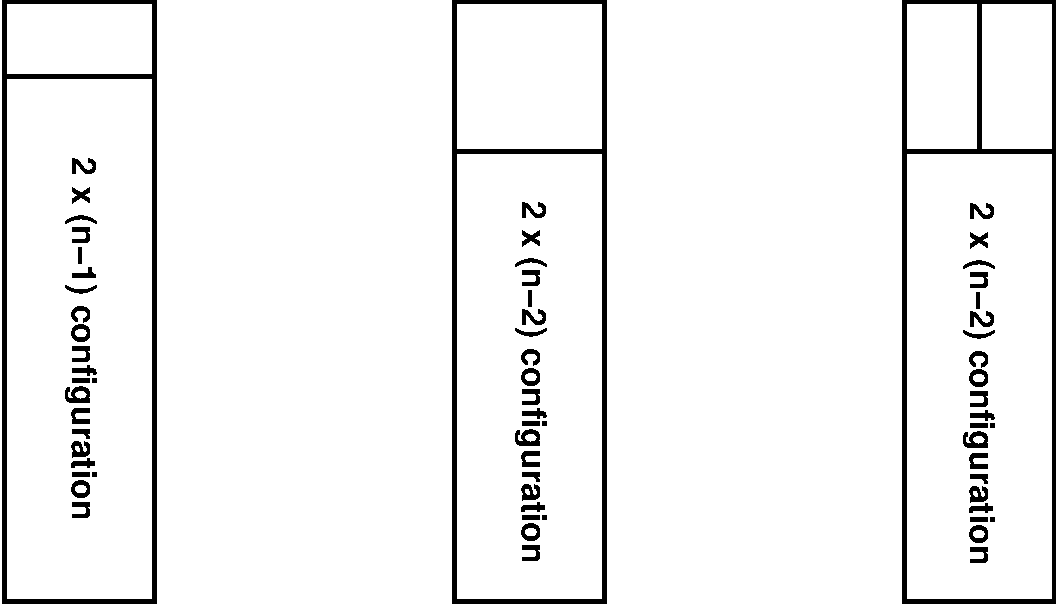
\includegraphics[height=2in]{rec2-types}}
\bigskip

\noindent There are $T_{n-1}$ winning configurations of the first
type, and there are $T_{n-2}$ winning configurations of the second and
third types.  Overall, the number of winning configurations on a $2
\times n$ board is:

\begin{eqnarray*}
T_n & = & T_{n-1} + 2 T_{n-2}
\end{eqnarray*}
\end{solution}

\problempart Use the Well Ordering Principle to prove that the number
of winning configurations on a $2 \times n$ Mini-Tetris board is:

\begin{eqnarray*}
T_n & = & \frac{2^{n+1}+(-1)^n}{3}
\end{eqnarray*}

\begin{solution}
\TBA{Revise for Well Order}

The proof is by strong induction on $n$, with the induction
hypothesis $T_n = (2^{n+1}+(-1)^n) / 3$.  The hypothesis is true for
$n = 1$ and $n = 2$, since we determined above that $T_1 = 1 =
(2^{1+1}+(-1)^1)/3$ and $T_2 = 3 = (2^{2+1}+(-1)^2)/3$.

Now suppose $n \geq 2$ and assume that the hypothesis holds for all $k
< n$.  Starting from the equation derived in the preceding problem
part, we have:

\begin{eqnarray*}
T_n	& = &	T_{n-1} + 2 T_{n-2} \\
 	& = &	\frac{2^n+(-1)^{n-1}}{3} +
		2 \cdot \frac{2^{n-1}+(-1)^{n-2}}{3} \\
	& = &	\frac{2^n-(-1)^n}{3} +
		\frac{2^n+2(-1)^n}{3} \\
	& = &	\frac{2^{n+1}+(-1)^n}{3}
\end{eqnarray*}

\noindent We use the induction hypothesis twice in the second step,
and then simplify in the third and fourth steps.  This completes the
inductive step.  By strong induction, the hypothesis holds for all $n
\geq 1$.  
\end{solution}

\end{problemparts}

\end{problem}

\endinput
